\begin{figure*}[tbh]
    \centering
    \begin{subfigure}{0.42\textwidth}
        \centering
        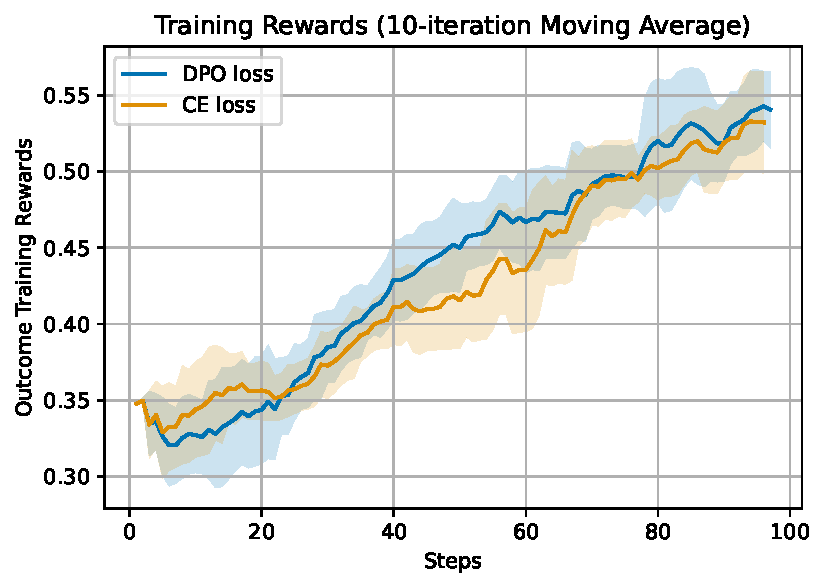
\includegraphics[width=\linewidth]{figures/images/train_rewards_dpo_vs_ce.pdf}
        \caption{Outcome training rewards.} % 第一个图形的子标题
        %\label{fig:train_rewards}
    \end{subfigure}
    \hfill % 在两个子图之间添加一些水平间距
    \begin{subfigure}{0.57\textwidth}
        \centering
        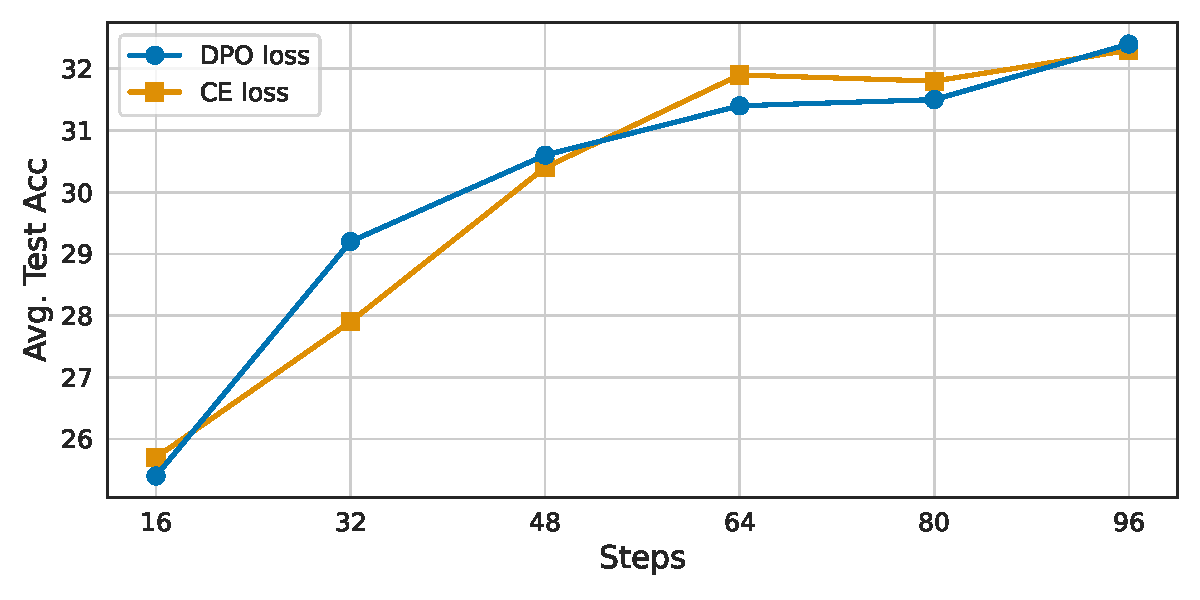
\includegraphics[width=\linewidth]{figures/images/dpo_vs_ce.pdf}
        \caption{Math test accuracy across different gradient steps.} % 第二个图形的子标题
        %\label{fig:test_accuracy}
    \end{subfigure}
    \caption{Outcome rewards and test accuracy of updating PRM with DPO or CE loss during training.} % 整个图形的标题
    \label{fig:dpo_vs_ce}
\end{figure*}